\documentclass[journal]{IEEEtran}
\usepackage{amsmath,amssymb,amsfonts}
\usepackage{tabularx}
\usepackage[utf8]{inputenc} % allow utf-8 input
\usepackage[T1]{fontenc}    % use 8-bit T1 fonts
\usepackage{url}            % simple URL typesetting
\usepackage{booktabs}       % professional-quality tables
\usepackage{amsfonts}       % blackboard math symbols
\usepackage{nicefrac}       % compact symbols for 1/2, etc.
\usepackage{microtype}      % microtypography
\usepackage{graphicx}
\usepackage{float}
\restylefloat{table}
\usepackage{hyperref}
\usepackage{multicol}
\usepackage{caption}
\usepackage{subcaption}
\usepackage{amsmath}
\usepackage{algorithm}
\usepackage{algpseudocode}
\usepackage{tikz}
\usetikzlibrary{trees}
\usepackage{listings}

\DeclareMathOperator*{\argmax}{arg\,max}  % in your preamble
\DeclareMathOperator*{\argmin}{arg\,min}  % in your preamble

\usepackage{textcomp}


%\usepackage[retainorgcmds]{IEEEtrantools}
%\usepackage{bibentry}
\usepackage{xcolor,soul,framed} %,caption

\usepackage[noadjust]{cite}
%\usepackage{biblatex}
%\bibliographystyle{plain}

\usepackage[font=small]{caption}

%=== TITLE & AUTHORS ====================================================================
\begin{document}
\bstctlcite{IEEEexample:BSTcontrol}
    \title{test}
\title{Accelerate Reinforcement Learning with Active Boundary}

\author{ Zongqiang Pang, Liping Bai ~\IEEEmembership{Member,~IEEE,} \thanks{Nanjing Unversity of Posts and Telecommunications, College of Automation \& College of Artificial Intelligence, Nanjing, Jiangsu,210000 China email:zqpang@njupt.edu.cn}}
% ====================================================================
\maketitle
% === ABSTRACT ====================================================================
% =================================================================================
\begin{abstract}
Reinforcement learning is not a new subject, yet with the advent of deep learning and fast GPU compuation, the world finally gets a glimpse into what is attainable with RL. Despite the routinely achieved jaw-dropping results, the blatant inefficiency embedded in RL methodologies can no longer be ignored should its full potential be realized. That is the focus of current research effort. We propose a new angle of attack which differs from that of RL researchers, who focus on driving out inefficiency with statistical tactics, and that of control researchers, who focus on merging RL with exisiting control methods. If there are techniques that humans utilize to accelerate our learning, why not apply the same to reinforcement learning agents? That is the basis of our proposed active boundary method. In this paper, we devised and implemented "Active Boundary for Reinforcement Learning Agents" based on our observations of the athletic training process. We conducted experiments in OpenAI Gym environments and concluded from the data that when the boundary is too restrictive, it hinders rather than facilitates the learning process. Yet when the boundary is set at its goldilocks spot, agent training can be accelerated, in some cases significantly, while yielding uncompromised training results. We believe our research is an important proof of concept that human training techniques can be successfully adopted by reinforcement learning process. This could open doors to future researches which tap into the rich reservoir of atheletic training tactics. All the code and data can be found at: \href{https://github.com/BaiLiping/ActiveBoundary}{github.com/BaiLiping/ActiveBoundary}
\end{abstract}
% === KEYWORDS ====================================================================
% =================================================================================
\begin{IEEEkeywords}
Reinforcement Learning, Reward Engineering, Accelerated Learning
\end{IEEEkeywords}
\IEEEpeerreviewmaketitle
% === I. Paper =============================================================
% =================================================================================
\section{Introduction}
\IEEEPARstart{R}{einforcement} learning (RL) is the process of methodically extracting information from data, gradually bounding policy distributions to maximize the expected reward along a sequence of actions. While RL researchers routinely generate paradigm-shifting results \cite{Mnih2013PlayingAW}\cite{Hausknecht2015DeepRQ}\cite{Andrychowicz2020LearningDI}\cite{Kalashnikov2018QTOptSD}\cite{Lee2020LearningQL}, there are aspects of RL that are inherently unreasonable and inefficient. I have yet to meet a child who learns to walk by exhaustively searching all the combinations that his joints can be move together, scoring each combination with the observed outcome, yet that is how RL agents pick up their control cues. If RL were to be successfully applied in real world situations, all these inefficiencies have to be squeezed out in one way or another, and that is indeed the focus of the current research effort. 

Two groups of researchers attack the problem from two different perspectives. RL researchers who are well versed in statistics and information theories approach the problem by devising ever more sophisticated statistical processes to maximize information extraction. Imitation learning and reverse reinforcement learning aim at automatically derive control strategy from demonstrated best solution\cite{Ho2016GenerativeAI}\cite{Peng2018DeepMimicED}\cite{Paine2018OneShotHI}\cite{Peng2020LearningAR}; Unsupervised learning, curiosity-driven learning hope to train agents with intuitions of the physical world\cite{Finn2016UnsupervisedLF}\cite{Pathak2017CuriosityDrivenEB}\cite{Burda2019LargeScaleSO}; Meta-Learning hopes to extract the overarching structures embedded in similar tasks so the control strategies would be applicable cross multiple problems\cite{Finn2017ModelAgnosticMF}\cite{Mishra2018ASN}; Hierarchical Reinforcement Learning seeks to decompose a task into its hierarchical subcomponents and accelerate the learning by exploiting the hierarchical structure\cite{Nachum2018DataEfficientHR}\cite{Vezhnevets2017FeUdalNF}; Bayesian Neural Network is used to measure the uncertainly of the model and avoid overfitting\cite{Blundell2015WeightUI}\cite{Gal2017ConcreteD}. Causal Reinforcement Learning builds on the idea of causal inference, hoping to accelerate agent training by exploiting the embedded causal relations.\cite{Dasgupta2019CausalRF}\cite{Zhang2020DesigningOD}

Control researchers who are capable of wielding control theories and optimization techniques can provide a systematic perspective to RL which is a dearth of analytical tools. One surprising area that controls researchers have contributed to reinforcement learning is the analysis of neural networks. DNN can be seen as a dynamic system and analyzed accordingly\cite{Weinan2017APO}\cite{Dupont2019AugmentedNO}. Optimizers are also empirically derived and lack theoretical underpinning. Control theorists also proposed possible geometrical ways to look at this problem \cite{Betancourt2018OnSO}. Regularized regression, which is a topic of research in statistical learning, can be seen as the dual problem of the primal constrained optimization. This dual perspective can be valuable addition to RL\cite{Nachum2020ReinforcementLV}\cite{Luo2019ADR}. The theoretical integration of control theory and reinforcement learning is likely to evolve further as time progresses. Another area where control theory and RL can merge is the combination of known control strategies with the data-driven approach. Instead of mathematically derive the differential equation, one can simply feed a DNN with sequential data\cite{Wu2020DataDrivenDL}. This approach is even more powerful in the spectral space\cite{Li2020FourierNO}. Neural Lander team of Caltech \cite{Shi2019NeuralLS} complimented classical control techniques with reinforcement learning to better handle the residual dynamics that elude traditional methods. Neural networks can also be complicated with a functional layer such as a known model\cite{Hewing2020LearningBasedMP}\cite{Mohan2020EmbeddingHP}\cite{Lusch2018DeepLF}, or a layer of differential solvers \cite{Bai2019DeepEM}\cite{BelbutePeres2020CombiningDP}. 

We propose an additional angle of attack for increasing RL efficiency based on our observations of how humans train. Professional athletes don't get where they are via trial-and-error. Their skillsets are forged through a series of theoretically and empirically proven training techniques that seek to maximize training efficiency. In this paper, we focus on one such technique: active boundary.

The objective of an active boundary is to facilitate data collection on critical states, much like a coach guides athletes towards experience with essential states instead of repeating steps that pave the way. We ascribe the observed training acceleration brought about by the active boundary method to this expedited data collection on critical states. We would elaborate on our ideas further in the subsequent sections.

We implemented the proposed active boundary scheme on various OpenAI Gym environments as a proof of concept and we concluded that when the boundaries are set appropriately, accelerated learning can be achieved and the resulting agents have indistinguishable evaluation scores compare to the agents trained with normal methods. We have confidence in our conclusion since while randomness might underline one set of data, it is highly unlikely that randomness alone can explain the same observations made in a different set of experiments. Our result indicated the feasibility of adopting human training techniques into RL setup and could be the beginning of other fruitful researches in this direction.

In section II we introduce reinforcement learning in the language of control. In section III we detail our proposed active boundary scheme for accelerated RL agent training. In section IV, we present the results of all our experiments. While the experiments are conducted in OpenAI Gym simulated environment, we consciously designed things in a way such that it can be conveniently implemented in the physical world as well. In the final section, we conclude what we have learned from our experiments and layout directions for further research.

\section{Reinforcement Learning For Control Researchers}

\subsection{Note on Notation and Nomenclature}
The first barrier that stands between control researchers and RL is the jungle of notations. At this point, just about every researcher has his own symbolic system. As noted by Warren Powell in his 2014 introductory paper on Approximate Dynamic Programming: "Somewhat frustratingly, these communities have also developed different vocabularies and different notational systems." Yet in the same breath, Powell introduced a new set of customized notation. \cite{Powell2009WhatYS} Here, we merely try to point out the differences to make life easier for control researchers. Control communities use the notation system introduced by Lev Pontryagin. The state is denoted by $ \mathcal{X}$, conventionally a letter representing the unknown. Action is denoted by $\mathcal{U}$, the first letter of Russian for action. The dynamics and stochasticity is captured by physical model constraints $x_{t+1}=f(x_t,u_t,e_t)$ where e denotes the noise of a system. The objective is usually to minimize the cost function $\mathcal{J(.)}$. Reinforcement Learning communities adapt their notation system from the field of Operations Research. State is denoted $\mathcal{S}$, Action is denoted $\mathcal{A}$. The system dynamics and stochasticity is captured via transition matrix $\mathcal{P}$ of a Markov Decision Process. The objective of RL is the maximize the reward function $\mathcal{R(.)}$. 

Richard Sutton uses terminologies that can be overloaded and confusing such as Monte Carlo, Temporal Difference(TD), in his book Introduction to Reinforcement Learning \cite{Sutton1998IntroductionTR}. Although the control community also has to deal with the sequential aspect of a problem, the terminologies there is much more down-to-earth and straightforward, such as one-step look ahead, n-steps look ahead. In the context of RL, Monte Carlo simply means update with data collected from an entire episode. Temporal Difference means update with data collected with one step. TD($\lambda$) means update with data collected with $\lambda$ steps. 

\subsection{From Optimization To Learning}

Reinforcement Learning is not a new subject, control researchers probably know it by the name Approximate Dynamic Programming (ADP) or Neuro Dynamic Programming (NDP). When the first batch of reasonable RL results was introduced, it was met with coldness by people in control. The preface of Bertseka's book Neuro Dynamic Programming provides a good sample of how reinforcement learning is perceived by the control community back in 1996: "...These methods (Reinforcement Learning) were aiming to provide effective suboptimal solutions to complex problems of planning and sequential decision making under uncertainty, that for a long time were thought to be intractable. Our first impression was that the new methods were ambitious, overly optimistic, and lacked a firm foundation...Three years later, after a lot of study, analysis, and experimentation, we believe that our initial impressions were largely correct." \cite{Bertsekas1996NeuroDynamicP}

Today, the theoretical foundation of RL is as bleak as it was in 1996, but its deficiencies can be easily papered over with the ever more impressive computational capacities. Before 2010, the predominant function approximators are handcrafted kernels, where feature spaces transform nonlinear functions into linear space. Today, the default function approximator is neural networks. Another major change in computation is that of GPU based parallelization. GPU programming uses to require a Ph.D. in computer graphics. Today, anyone who is proficient in C/C++ can program GPU to parallelize their computation with CUDA\cite{Nickolls2008ScalablePP}. Software packages such as PyTorch\cite{Paszke2017AutomaticDI} and Tensorflow\cite{Abadi2016TensorFlowAS} made this even more trivial.

In order to better introduce RL to control researchers, we built on Benjamin Recht's presentation\cite{Recht2018ATO}, framed RL in the language of optimization. Reinforcement Learning is an umbrella term, which encompasses distinctive genres of learning. Learning in the context of RL means updating parameters of the function approximators. Categorically speaking, there are three avenues where learning finds its way into optimization as shown in Figure\ref{fig:1}. 
\begin{figure}
    \centering
    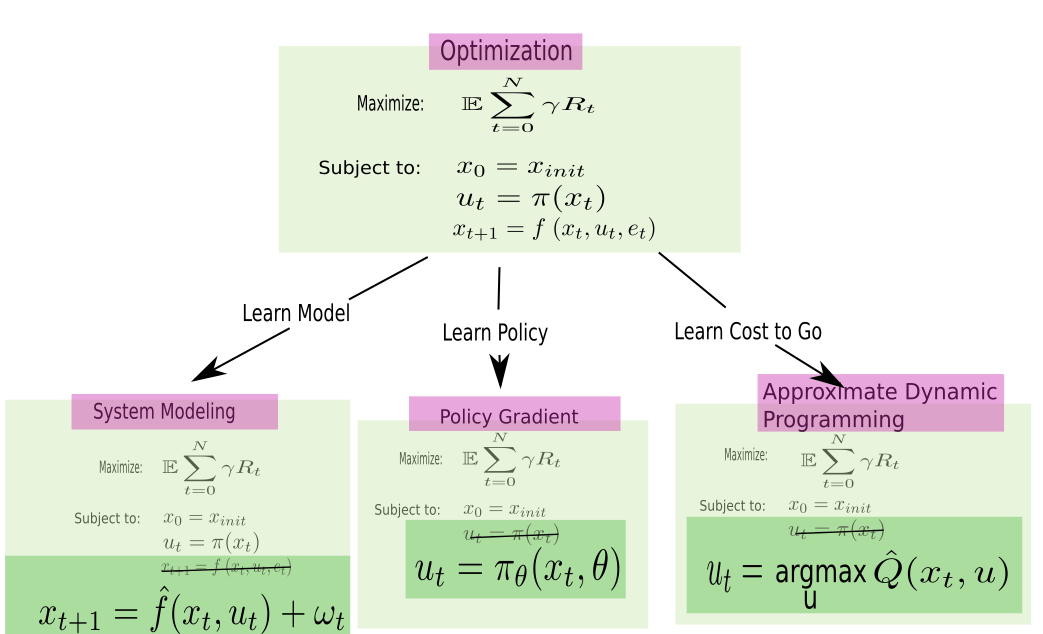
\includegraphics[width=0.5\textwidth]{Control.png}
    \caption{From Optimization to Learning}
    \label{fig:1}
\end{figure}

Model-Based or Model-Free learning refers to whether or not learning is used to approximate the system dynamics function. If there is an explicit action policy, it is called on-policy learning. Otherwise, the optimal action would be implicitly captured by the Q value function and that would be called off-policy learning instead. Importance sampling allows "limited off-policy learning" capacity, which allows data reuse in a trusted region. Online learning means interleaving data collection and iterative network parameters update. Offline learning means the data is collected in bulk first and then the network parameters are set with regression computation. Batch learning, as the name suggested, is in between online and offline learning. An agent would first generate data that fill its batch memory and then sample from the batch memories for iterative parameter update. New data would be generated with the updated parameters to replace older data in the memory. This taxonomy is somewhat outdated now. When Richard Sutton wrote his book, the algorisms he had in mind fall nicely into various categories. Today, however, the popular algorisms would combine more than one route to derive superior performance, and can't be pigeonholed.

We will not go into the details of various RL algorithms and the zoo or acronyms that come with it, as that is beyond the scope of this paper. PPO agents were chosen for all our experiments because the learning curves generated by PPO agents are smoother compare to other agents. The goal of our paper is to indicate the proposed active boundary method works, which is easier to be shown with smoother curves. However, we would like to point out two crucial concepts that undergird the feasibility of reinforcement learning.

\subsubsection{Bellman Update}

Reasoning backward or Dynamic Programming forms the basis of reinforcement learning. If we know the desired final state and system dynamics then we can simply compute backward on the penultimate step. Set the penultimate step as the final step, then repeat the process until the action strategy for the initial state is obtained. This approach, Bellman Update, would work if two prerequisites are met: first, the system dynamics function is known; second, the dimensions of observation space and action space are small. Neither would be true for the problems we encounter in the real world.

When the dynamics are unknown yet the dimensions of the problem are manageable, the cost-to-go lookup table can be constructed with sampling methods. As mentioned earlier, the way that the lookup table is updated with the sample can be categorized by the horizon of the data collection. If the lookup table is updated with data collected from an entire episode, it is called the Monto Carlo method. If the lookup table is updated every step, it is called Temporal Difference method, and there are various methods in between these two extremes. When the dimensions of the problem are large in addition to unknown dynamics, function approximators are used for the system model, the policy function, or the cost-to-go function. 

Immediately, control researchers can spot the deficiency with the latter case. For backward reasoning to work properly, the notion of optimality has to be satisfied either through known dynamics function or robust sampling methods, yet when the dynamics are unknown and the dimensions large, the notion of optimality can no longer be guaranteed through sampling. This is where the expertise of statisticians and information theories comes in and the research topic of exploration-exploitation trade-off.

\subsubsection{Bootstrap}

Another fundamental concept for RL is convergence through bootstrap. Instead of asymptotically approaching a known target function, bootstrap methods approach an assumed target first and then update the target assumption based on collected data. This process is illustrated by Figure\ref{fig:bootstrap}. Intuitively, when estimation functions are evaluated with assumption instead of the true value, things could just run around in circles and never converge. That is indeed the case before the introduction of DQN\cite{Osband2016DeepEV}. As a matter of fact. the stability and convergence achieved in that paper are more of a reflection on the techniques and know-how of the DeepMind team. Initially, those results can not be easily replicated by other labs. Even today, instability in RL is still a major research focus. 

\begin{figure}
\centering
\begin{subfigure}{0.25\textwidth}
  \centering
  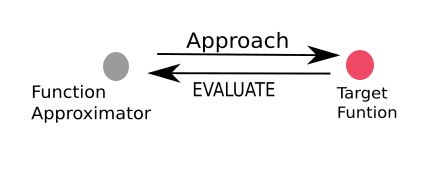
\includegraphics[width=\linewidth]{onego.png}
  \caption{With Known Evaluation Function}
\end{subfigure}%
\begin{subfigure}{.25\textwidth}
  \centering
  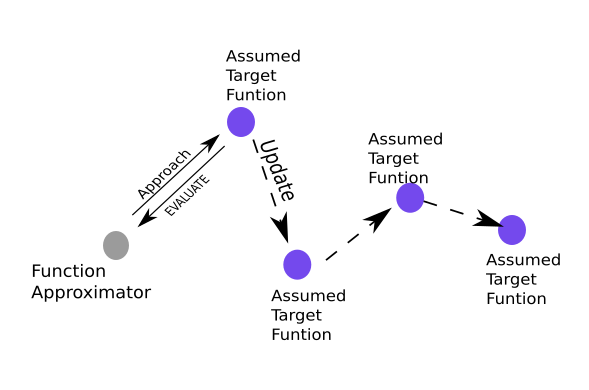
\includegraphics[width=\linewidth]{bootstrap.png}
  \caption{Bootstrap}
\end{subfigure}
\caption{Convergence through Bootstrap}
\label{fig:bootstrap}
\end{figure}


\section{Expedited Data Collection on the Critical States with Active Boundary}
As we pointed out in the introduction, human has amassed vast amounts of empirically proven techniques for accelerated skill acquisition. In this paper, we focus on the idea of expedited data collection on critical states with active boundaries, where critical states refer to the ones that are essential for skill acquisition.

Focused training with critical states is the bread and butter for athletes. Chess players start their training with endgames because that allows them to dwell on critical steps which illustrate the reasoning behind chess tactics, instead of wasting time on the "mechanical/maintenance moves" that lead up to a strategic position; Tennis coaches feed athlete balls with a specific angle and spin speed to force he with a backhand or forehand response. Examples like this are abundant in the world of sports. Active boundary is one way to implement focused training with critical states. 

When the athlete is about to fall, an attentive coach would apply force to course-correct on behalf of the athlete. This way, the athlete would have experienced the right way to handle that state as opposed to just falling. As indicated by Figure \ref{fig:athelete}, a coach can implement an active boundary because he can apply the appropriate force in due time. A safety net, on the other hand, is a passive boundary, since it does nothing other than catch people during a fall and no information on the critical state is generated in that process. The distinction between active and passive boundary is important because while prevention of premature termination is an implicit outcome of active boundary, it is by no means its primary goal. The protective property of active boundary stems from the fact that when a critical state is handled poorly, a terminal state would ensue. Therefore, the protective property is a by-product of directing the agents towards critical states. We would further accentuate the distinctions in the following section where we provide details of our implementation of active boundary. 

\begin{figure}
\centering
\begin{subfigure}{0.25\textwidth}
  \centering
  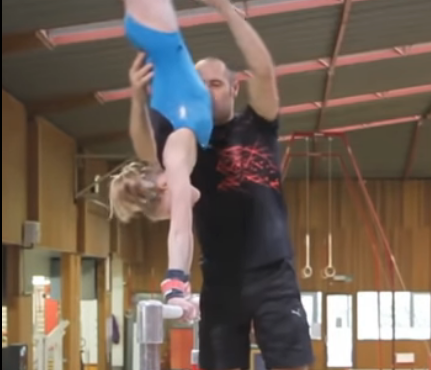
\includegraphics[width=\linewidth]{training1.png}
  \caption{Active Boundary}
\end{subfigure}%
\begin{subfigure}{.25\textwidth}
  \centering
  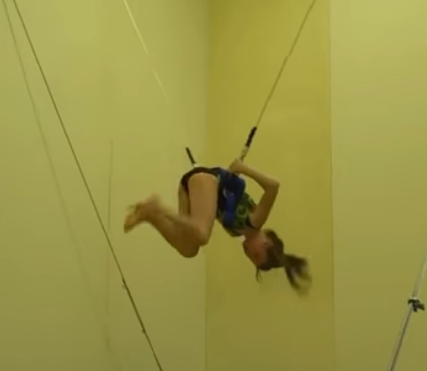
\includegraphics[width=\linewidth]{training2.png}
  \caption{Passive Boundary}
\end{subfigure}
\caption{Difference Between Active Boundary and Passive Boundary}
\label{fig:athelete}
\end{figure}

\section{Implement active Boundary in OpenAI Gym}
We implemented our active boundary experiments in OpenAI Gym\cite{Brockman2016OpenAIG} as a proof of concept. We are cognizant of the fact that eventually, things should apply to a real-world scenario. Therefore, we designed the active boundary in a manner such that it can be swiftly adapted to physical implementation. Agents are implemented with tensorforce\cite{tensorforce}. We sorted out the observation space and action space for each environment and recorded them in the code of each experiment.

As we suggested in the previous section when agents reach the critical state, "correct actions" would be applied by the active boundary to the agent, hence the name "active". Much like a coach would guide athletes through the most crucial step of the training. We also designed a penalty term associated with active boundary to discourage its use. If the agent act flawlessly at the critical state, no penalty would be applied. On the other hand, if the agent requires active boundary intervention, a penalty term would be registered. 

The positions and penalty terms are set in an ad hoc fashion in our experiments. At this point, we do not have an analytical frame that can guide us in making such decisions. We choose three positions for the boundary during each experiment and 4-6 penalty terms ranging from 0 upwards. The rule of thumb we used for the penalty is that the punishment score should be comparable to the reward.

Our experiments are conducted over the following environments: CartPole, with discrete action space; Inverted Pendulum, with continuous action space; Inverted Double Pendulum; Hopper; Walker2D. We did not implement our approach to more sophisticated environments such as HalfCheetah, Humanoid, and HumanroidStandup due to hardware constraints. Yet we feel that for the data we collected, our approach has shown conclusive results. The following are our experiment setup and results.

The dashed black lines are the training results of agents with normal training, which functions as the control group and the benchmark. The colored lines are the results of agents trained with varying penalty terms. The average evaluation scores of the agents are presented at the upper left corner of the graph.

\subsection{CartPole and Inveretd Pendulum}
CartPole's Observation Space is the vector: [Cart Position, Cart Velocity, Pole Angle, Pole Angular Velocity]. The discrete action space for cartpole is: [Push Cart to the left, Push cart to the right]. The continuous action space for Inverted Pendulum is an action ranging from -1 to 1, where -1 means the actuator moves the cart to the left with maximum power and 1 means the actuator moves the cart to the right with maximum power. The maximum episode step number for cartpole and inverted pendulum are 500 steps and 300 steps respectively. The terminal state for cartpole is angle of absolute value greater than 24 degrees. The terminal state for the inverted pendulum is an angle of absolute value greater than 0.2 radius. The reward for cartpole and inverted pendulum are both 1 for each step and 0 for the terminal step. 

The active boundary is implemented as a ring anchored on the cart, at the height of the middle of the pole. Touch sensors would be installed in order to detect contact between the pole and the ring. We propose three sets of rings each allows a maximum angle of 0.5, 0.7, and 0.9 of the terminal state angle in the cartpole environment and 0.1, 0.4, 0.5 radii in the inverted pendulum environment, as shown by Figure \ref{fig:cartpolePB}. 

\begin{figure}
     \centering
      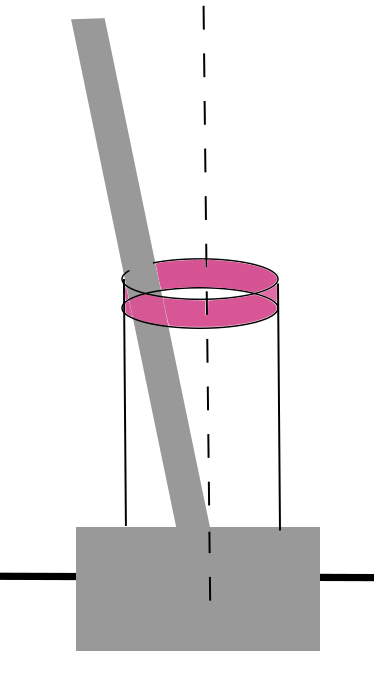
\includegraphics[width=0.1\textwidth]{cartpole1.png}
      \caption{CartPole/Inverted Pendulum active Boundary}
      \label{fig:cartpolePB}
\end{figure}
When contact between the pole and the active boundary is detected by the sensor, the cart would be pushed towards the appropriate direction depending on the sign of the angle. This step can be easily programmed by a microcontroller in physical implementation, and for implementation in simulation, it is just a matter of specifying a premeditated action. For detailed code, please refer to the code depository. Note that should the boundary is set without touch sensors and the corresponding actions, it would just be a passive boundary instead of an active one. 

A penalty term, which is chosen from vector [0,-5,-7,-10,-12,-15], would incur every time the pole contacts the active boundary. Our experiment result on cartpole are shown by Figure \ref{fig:CartPole}. The experiment result on inverted pendulum is shown by figure \ref{fig:InvertedPendulum}. As the data suggest, when the boundary is set too restrictively, it severely hinders the training. The best results is seen when the boundary is set at 10.8 degrees. After the agents are done training, we evaluate their performance in normal environments, the average evaluation scores are presented at the upper left part of the graphs. Our data suggest that during the evaluation, agents with accelerated training perform comparably to the agents with normal training.


\begin{figure}
    \centering
    \captionsetup[subfigure]{font=scriptsize,labelfont=scriptsize}
    \begin{subfigure}[b]{0.5\textwidth}
      \centering
      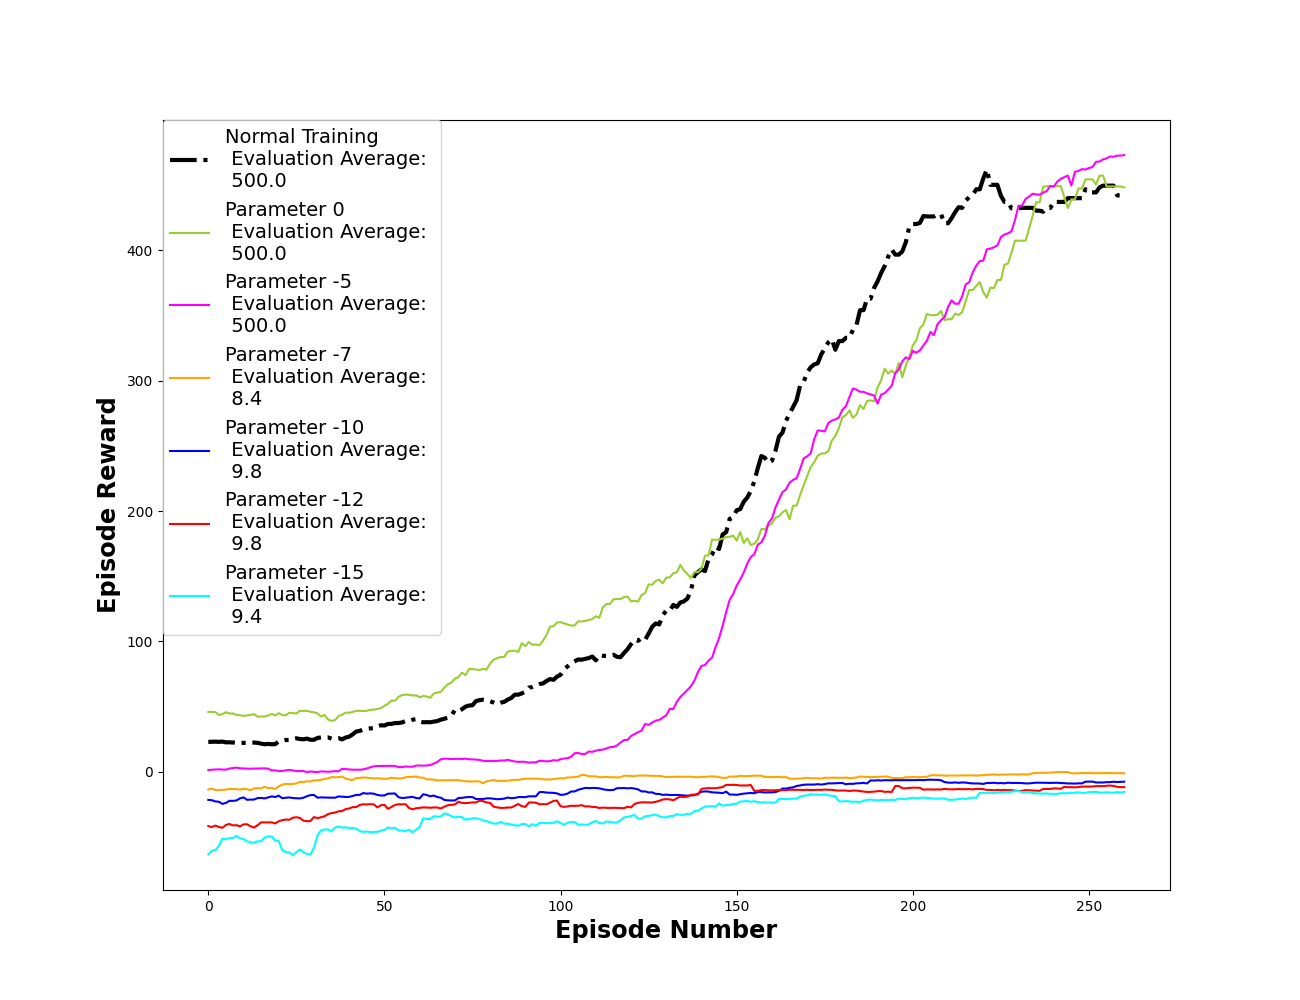
\includegraphics[width=\textwidth]{Cartpole_with_Boundary_at_0.5.png}
    \end{subfigure}
    \vspace*{0.0mm}
    \begin{subfigure}[b]{0.5\textwidth}
      \centering
      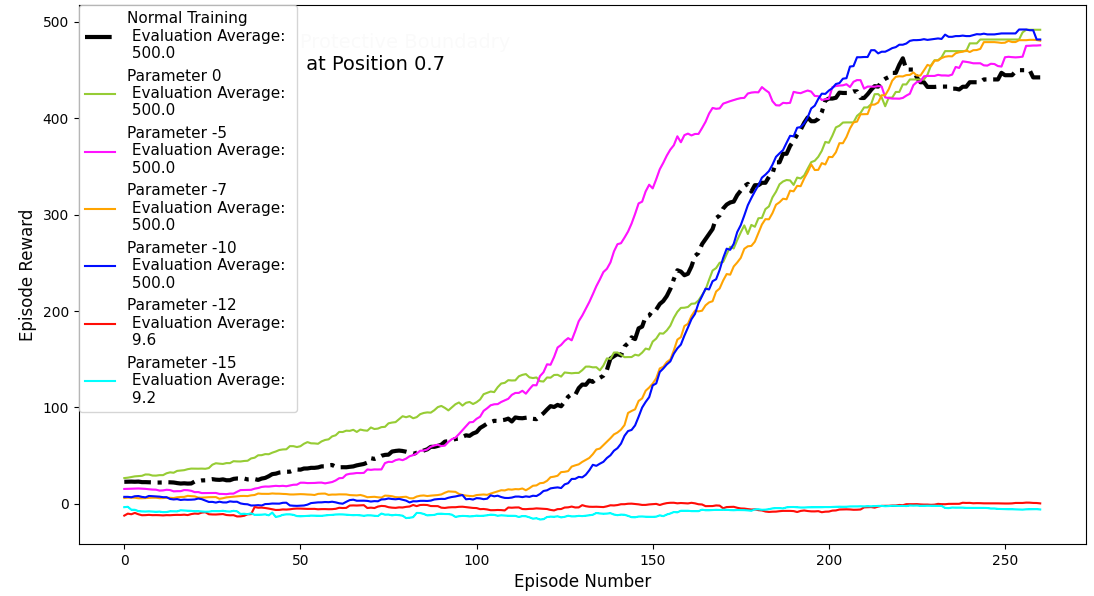
\includegraphics[width=\textwidth]{Cartpole_with_Boundary_at_0.7.png}
    \end{subfigure}
    \vspace*{0.0mm}
    \begin{subfigure}[b]{0.5\textwidth}
      \centering
      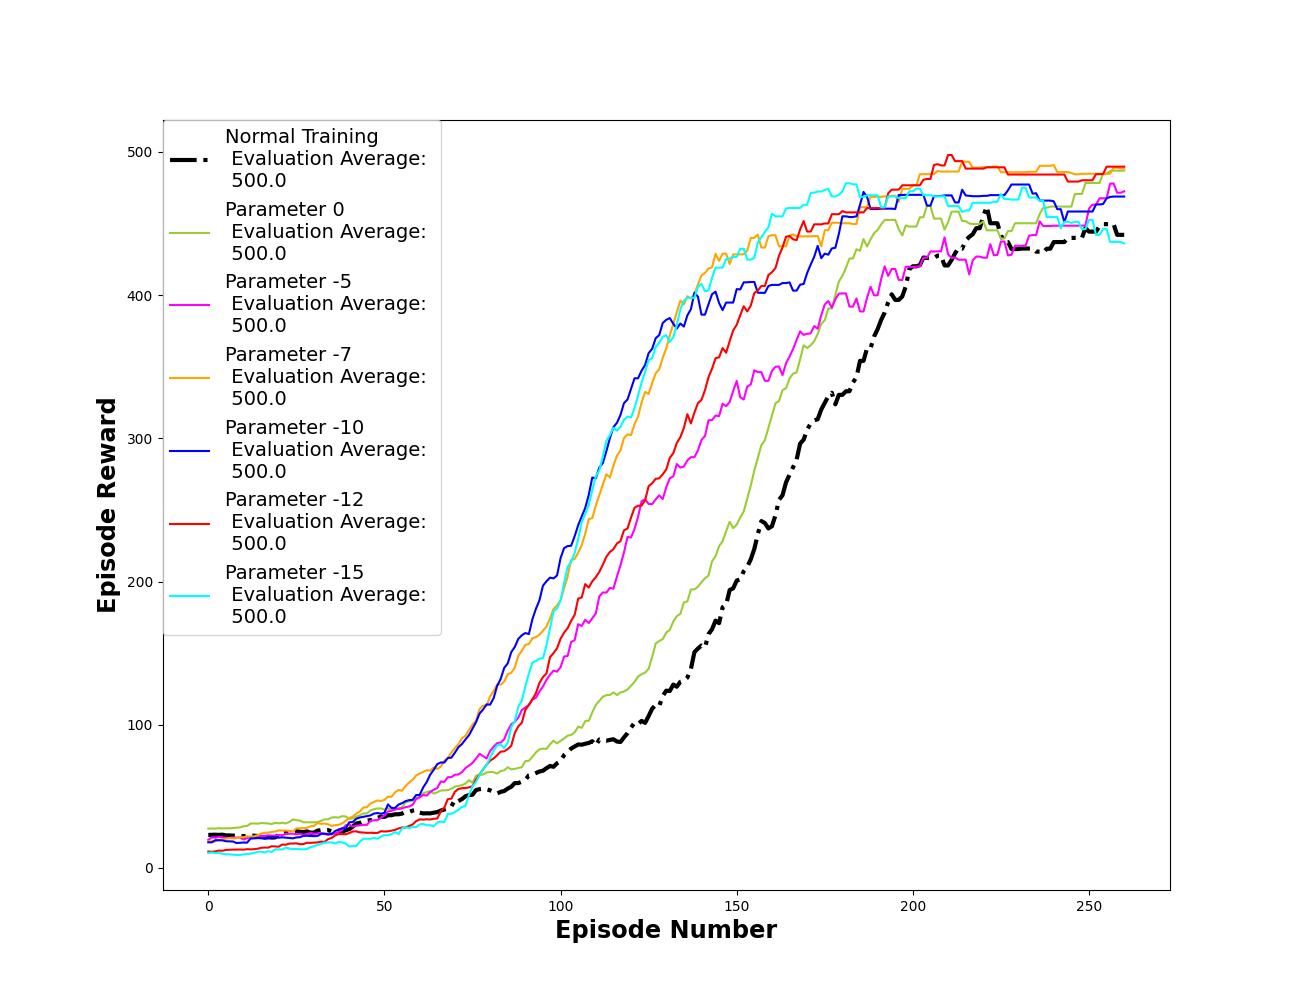
\includegraphics[width=\textwidth]{Cartpole_with_Boundary_at_0.9.png}
    \end{subfigure}
    \caption{CartPole Experiments}
    \label{fig:CartPole}
\end{figure}

\begin{figure}
    \centering
    \begin{subfigure}[b]{0.5\textwidth}
      \centering
      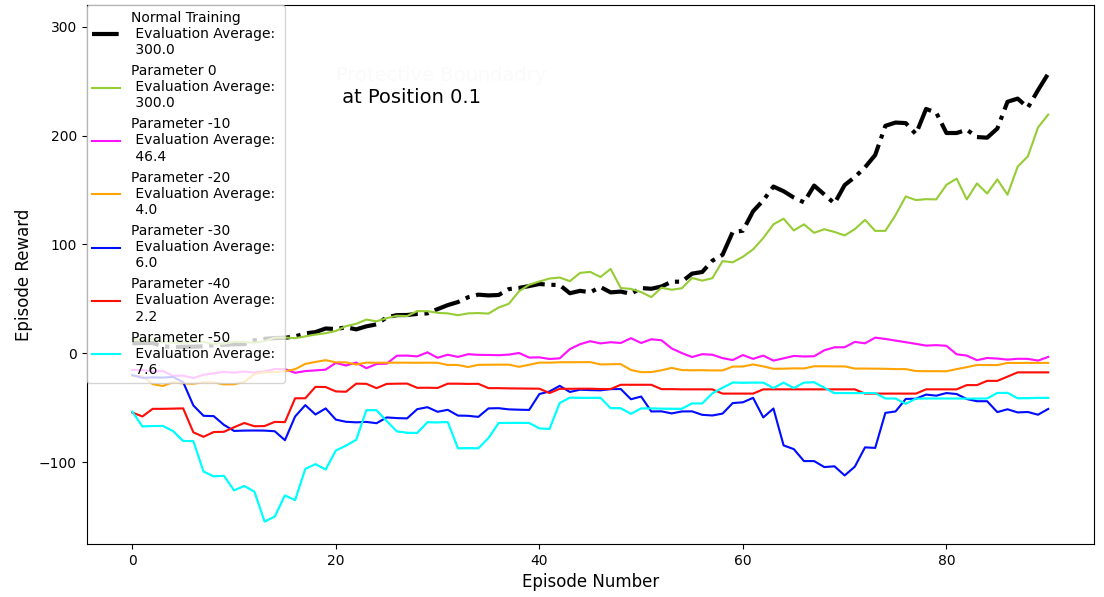
\includegraphics[width=\textwidth]{Inverted_Pendulum_with_Boundary_at_0.1.png}
    \end{subfigure}
    \vspace*{0.0mm}
    \begin{subfigure}[b]{0.5\textwidth}
      \centering
      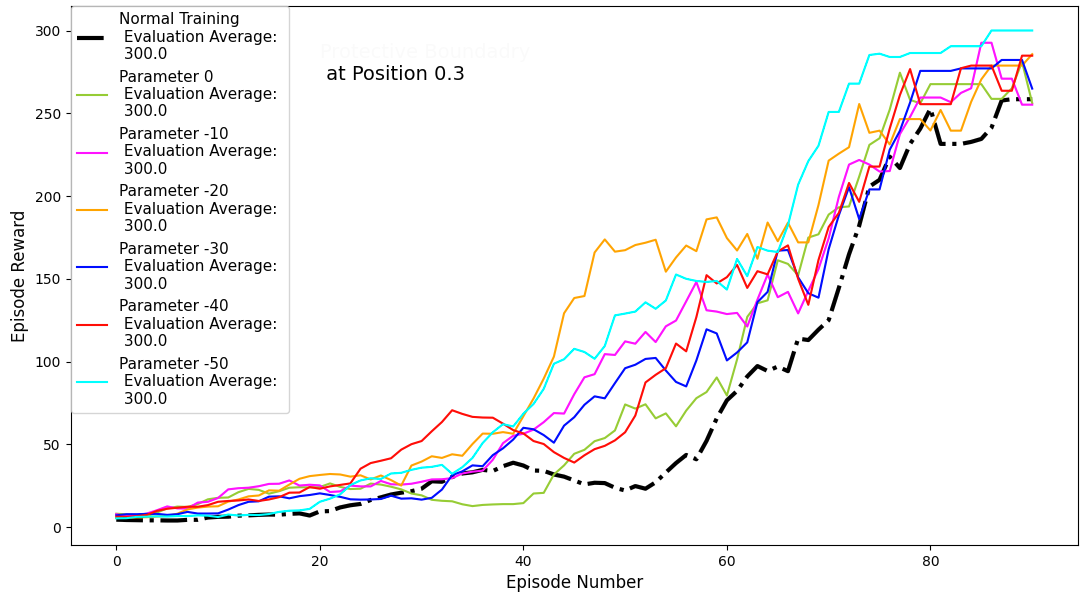
\includegraphics[width=\textwidth]{Inverted_Pendulum_with_Boundary_at_0.3.png}
    \end{subfigure}
    \vspace*{0.0mm}
    \begin{subfigure}[b]{0.5\textwidth}
      \centering
      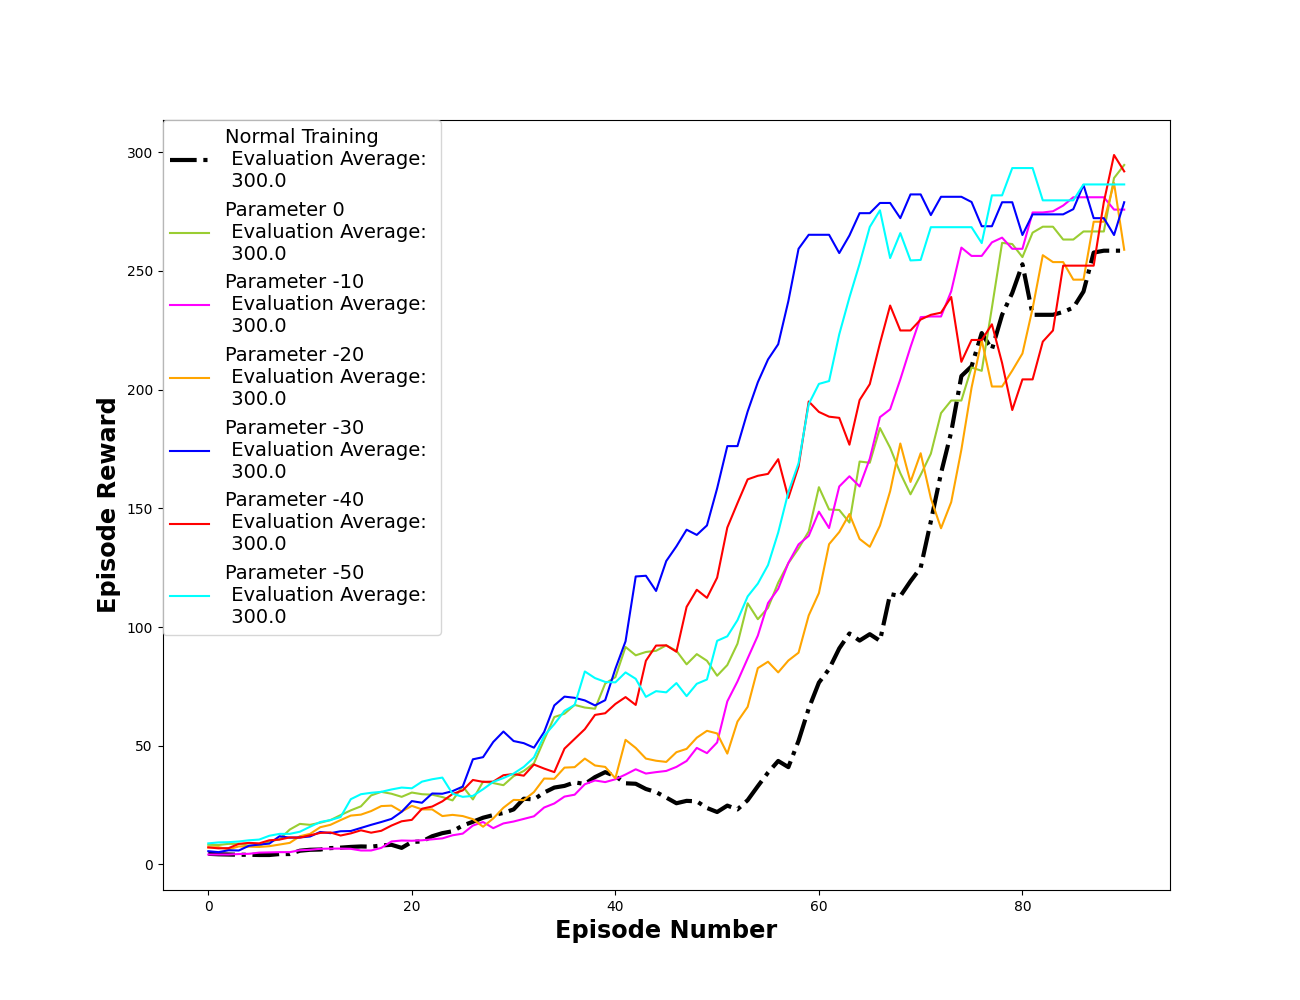
\includegraphics[width=\textwidth]{Inverted_Pendulum_with_Boundary_at_0.5.png}
    \end{subfigure}
    \caption{Inverted Pendulum Experiments}
    \label{fig:InvertedPendulum}
\end{figure}

\subsection{Inverted Double Pendulum}
The inveretd double pendulum has observation space of the following: [x position of the cart, sin($\theta_1$), sin($\theta_2$),cos($\theta_1$),cos($\theta_2$),velocity of x, angular velocity of $\theta_1$, angular velocity of $\theta_2$, constraint force on x, constraint force on $\theta_1$, constraint force on $\theta_2$]. $\theta_1$ and $\theta_2$ are the angles of the upper and lower pole perspectively.

The action space for Inverted Double Pendulum is an action ranging from -1 to 1, where -1 means the actuator moves the cart to the left with maximum power and 1 means the actuator moves the cart to the right with maximum power.

The Terminal state of double inveretd pendulum is when the y postion of the upper pole, which can not be observed by the agent, falls below 1.

We design the active boundary to be located at the same height as does the joint between the upper and the lower pole, as indicated by Figure \ref{fig:doublePB}. The boundary allows the joint to flex for 0.4, 0.5 and 0.6 radii respectively, each with the penalty parameters of a choice between 0,-3,-4,-5,-6,-7. When the joint extends to touch the active boundary, an action of -1 or 1 would be automatically applied to rectify the situation, depending on the sigh of the angles.

\begin{figure}
     \centering
      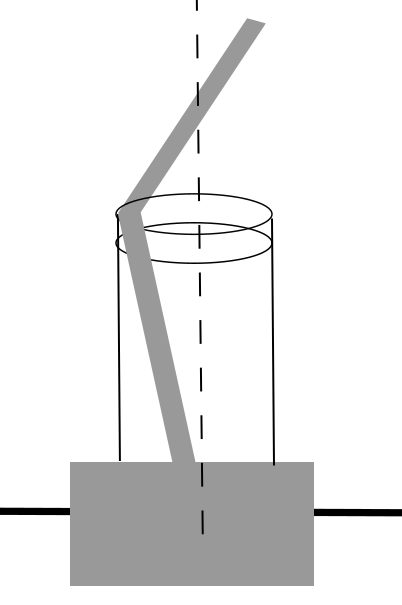
\includegraphics[width=0.1\textwidth]{cartpole2.png}
      \caption{Inveretd Double Pendulum active Boundary}
      \label{fig:doublePB}
\end{figure}

Our experiment result is shown by Figure \ref{fig:Double Pendulum}. The conclusion is similar to that of cartpole and inverted pendulum results. When the active boundary is set at 0.4 radii, it hinders learning rather than facilitate it. When the boundary is set at 0.5 radii with a penalty parameter of -7, we see the most drastic acceleration of agent training. However, when the boundary is set at 0.6 radii, it seems to have given the agent too much flexibility since the result suggests that the acceleration is not as profound compare to that of the boundary set at 0.5.

\begin{figure}
    \centering
    \begin{subfigure}[b]{0.5\textwidth}
      \centering
      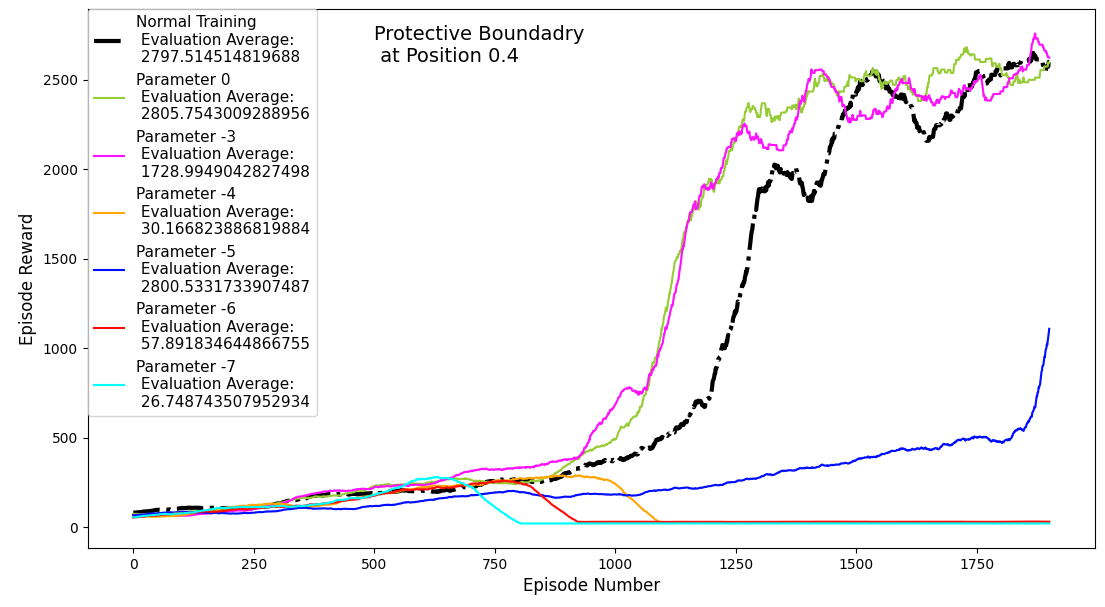
\includegraphics[width=\textwidth]{Double_Pendulum_with_Boundary_at_0.4.png}
    \end{subfigure}
    \vspace*{0.0mm}
    \begin{subfigure}[b]{0.5\textwidth}
      \centering
      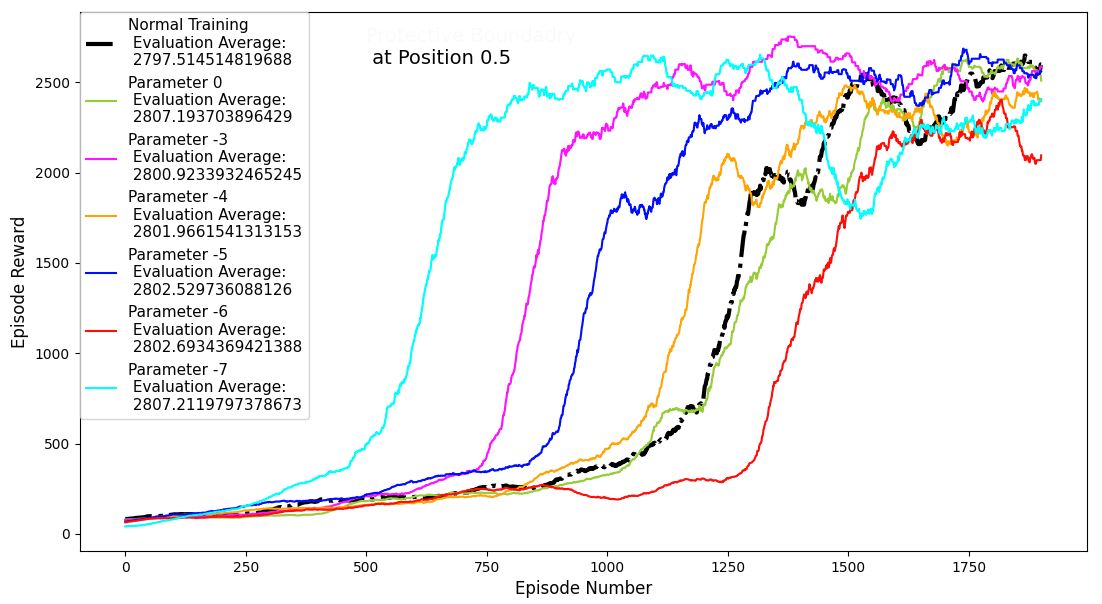
\includegraphics[width=\textwidth]{Double_Pendulum_with_Boundary_at_0.5.png}
    \end{subfigure}
    \vspace*{0.0mm}
    \begin{subfigure}[b]{0.5\textwidth}
      \centering
      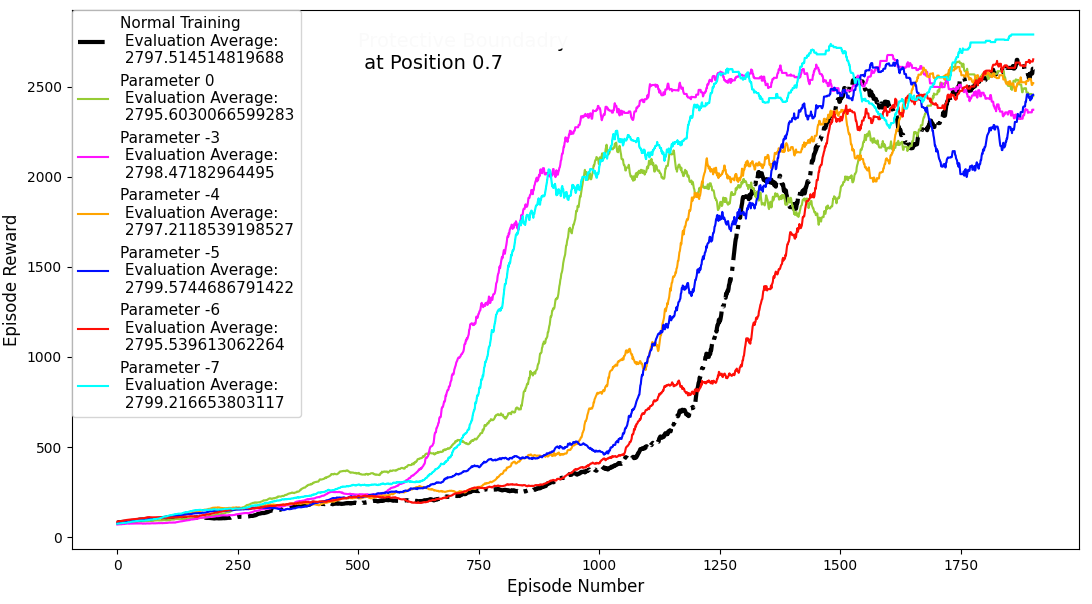
\includegraphics[width=\textwidth]{Double_Pendulum_with_Boundary_at_0.7.png}
    \end{subfigure}
    \caption{Inverted Double Pendulum Experiments}
    \label{fig:Double Pendulum}
\end{figure}


\subsection{Hopper}
The observation space of hopper is the following vector: [z position, y position, thigh joint angle, leg joint angle, foot joint angle, velocity at x-axis, velocity at z-axis, velocity at y-axis, angular velocity of thigh joint, angular velocity of leg joint, angular velocity of foot joint].

The action space of hopper are three continuous action choices for three actuators [thigh actuator, leg actuator, foot actuator]. The range of for actuators are -1, which means apply force towards the negative direction with maximum power, and 1 which means apply force towards the positive direction with maximum power.

The terminal states for hopper are when the absolute y position is greater than 0.2.

There are more than one ways to implement active boundary in hopper environment. Because we want things to be applicable in real-world scenarios, we chose the implementation with the easiest setup. In our experiment, the active boundary is defined with the y-position at 0.05, 0.1 and 0.15, each with the penalty parameters that is chosen from 0,-3,-5,-7,-10 as shown by Figure \ref{fig:hopperPB} When the agent touches the active boundary, we gently guide it slightly towards the center line, and the velocities terms are all set to zero. We seek to mimic how a coach would guide an athlete towards the desired trajectory during training. When the athlete is about to deviate off-course, the coach would take over and apply the appropriate force to slightly reset the trajectory. This can be implemented with an automatic harness in a physical experiment.

Our experiment result is shown by Figure \ref{fig:Hopper}. Similar to the conclusion drawn with previous data, when the active boundary is set too narrowly at 0.05 y position, it restricts the agent and almost completely halts the agent training. The best training acceleration is observed when the boundary is set at 0.15 y position.

\begin{figure}
     \centering
      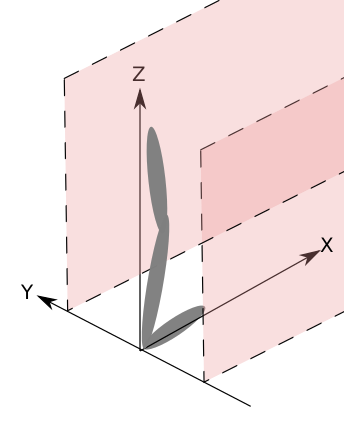
\includegraphics[width=0.2\textwidth]{hopper.png}
      \caption{Hopper active Boundary}
      \label{fig:hopperPB}
\end{figure}

\begin{figure}
    \centering
    \begin{subfigure}[b]{0.5\textwidth}
      \centering
      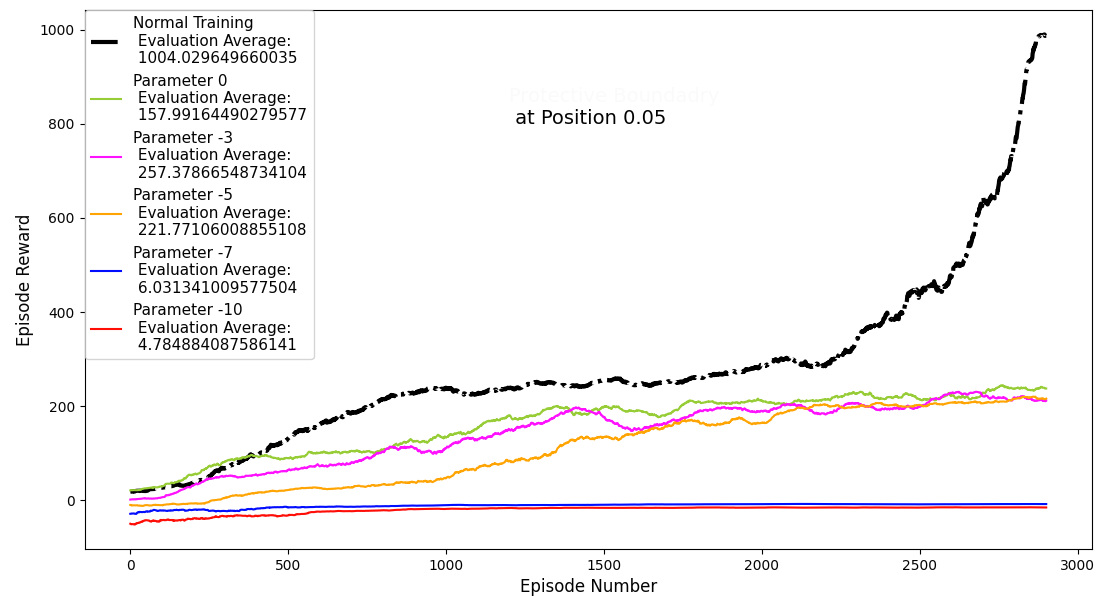
\includegraphics[width=\textwidth]{Hopper_with_Boundary_at_0.05.png}
    \end{subfigure}
    \vspace*{0.0mm}
    \begin{subfigure}[b]{0.5\textwidth}
      \centering
      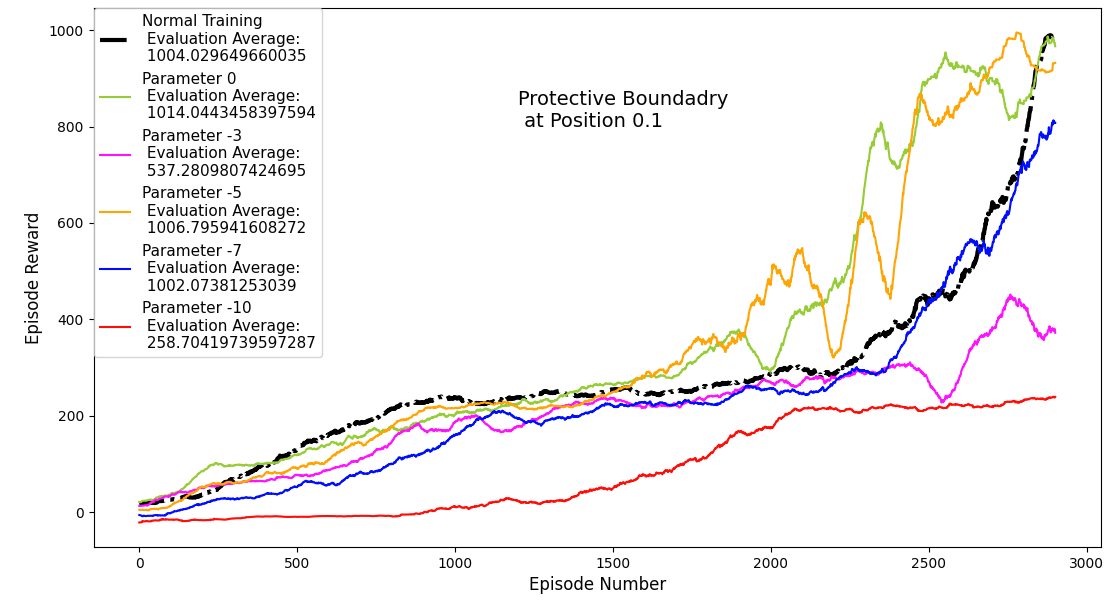
\includegraphics[width=\textwidth]{Hopper_with_Boundary_at_0.1.png}
    \end{subfigure}
    \vspace*{0.0mm}
    \begin{subfigure}[b]{0.5\textwidth}
      \centering
      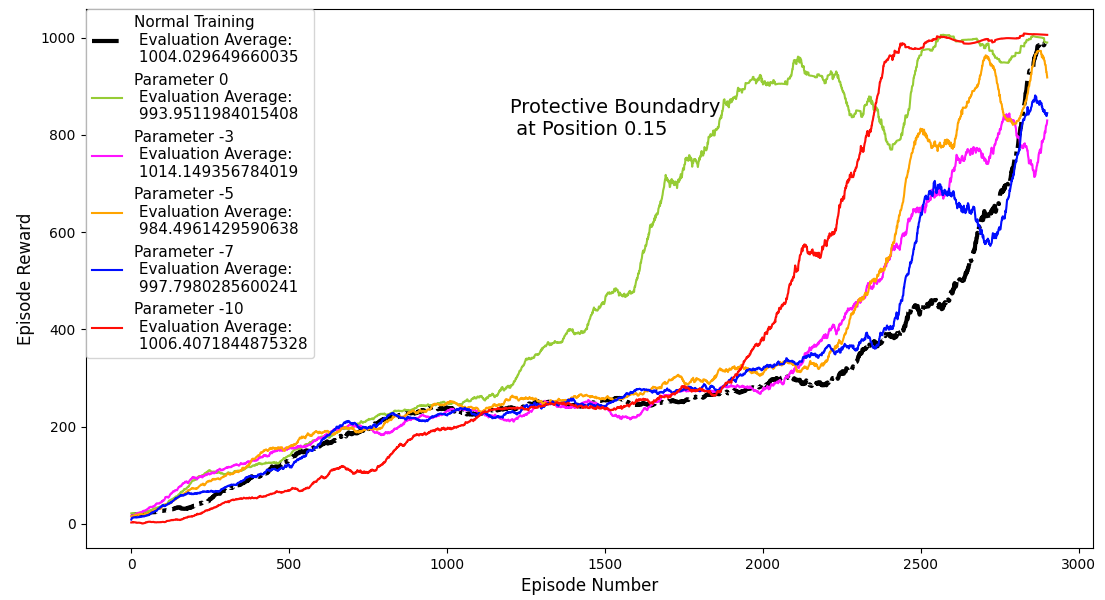
\includegraphics[width=\textwidth]{Hopper_with_Boundary_at_0.15.png}
    \end{subfigure}
    \caption{Hopper}
    \label{fig:Hopper}
\end{figure}


\subsection{Walker2d}
The walker environment's observation space is the following vector: [z position, y position, right thigh joint angle, right leg joint angle, right foot joint angle, left thigh joint angle, left leg joint angle, left foot joint angle, velocity along x axis, velocity along z axis, velocity along y axix, angular velocity for right thigh joint, angular velocity for right leg joint, angular velocity for right foot joint, angular velocity for left thigh joint, angular velocity for left leg joint, angular velocity for left foot joint]

There are 6 actuators for the right thigh joint, right leg joint, right foot joint and left thigh joint, left leg joint, left foot joint perspectively. The range for the motors is -1, which means apply force towards the negative direction with maximum power and 1, which means apply force towards the positive direction with maximum power.

The terminal states are when the z position falls below 0.8 or rise above 2 or the absolute value of y position is greater than 1.

The active boundary is set with the y position at 0.3, 0.7 and 0.9, each with the penalty parameters that is chosen from 0,-5,-10,-15,-20 as shown by Figure \ref{fig:walkerPB}. Similar to the active boundary for hopper, when the agent touches the active boundary in the walker environment, we gently guide it slightly towards the central line, and the velocities terms are all set to zero in the meantime.

Our experiment result is shown in Figure \ref{fig:Walker}. Yet again the experiment result suggests the same conclusion: when the boundary is positioned at 0.1, it acts as a barrier to training. When it is set at 0.7 positions, it could accelerate training with the appropriate penalty term.

\begin{figure}
     \centering
      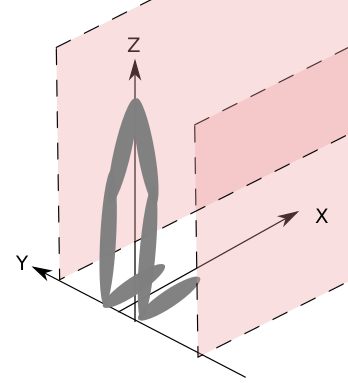
\includegraphics[width=0.2\textwidth]{walker.png}
      \caption{Walker2d active Boundary}
      \label{fig:walkerPB}
\end{figure}

\begin{figure}
    \centering
    \begin{subfigure}[b]{0.5\textwidth}
      \centering
      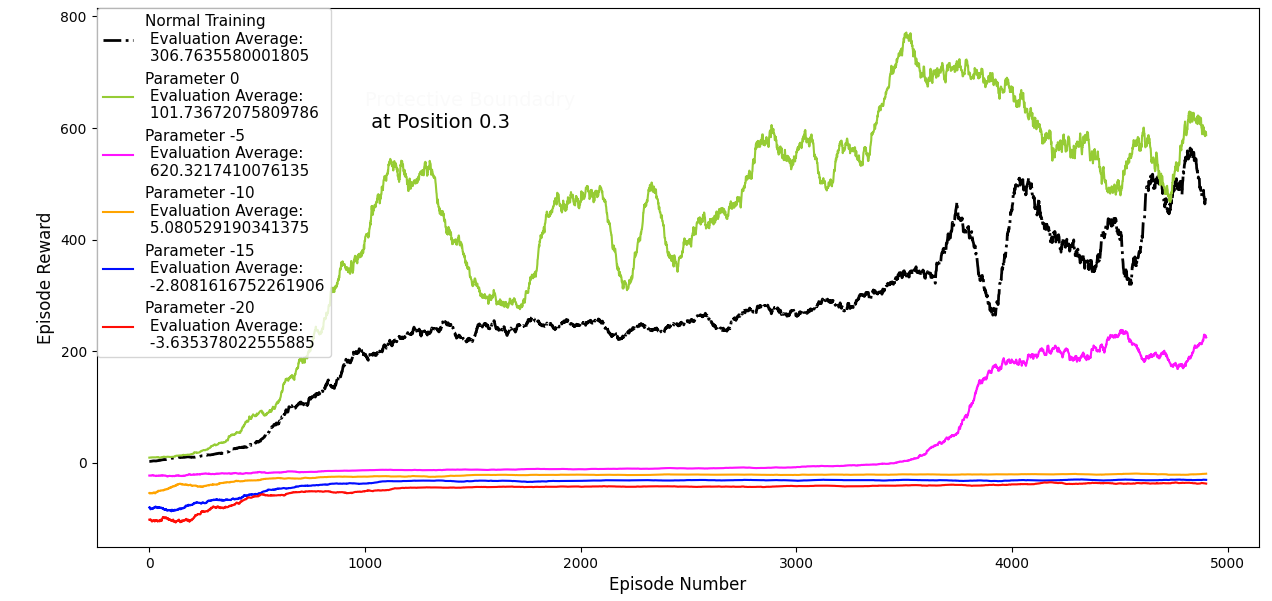
\includegraphics[width=\textwidth]{Walker_with_Boundary_at_0.3.png}
    \end{subfigure}
    \vspace*{0.0mm}
    \begin{subfigure}[b]{0.5\textwidth}
      \centering
      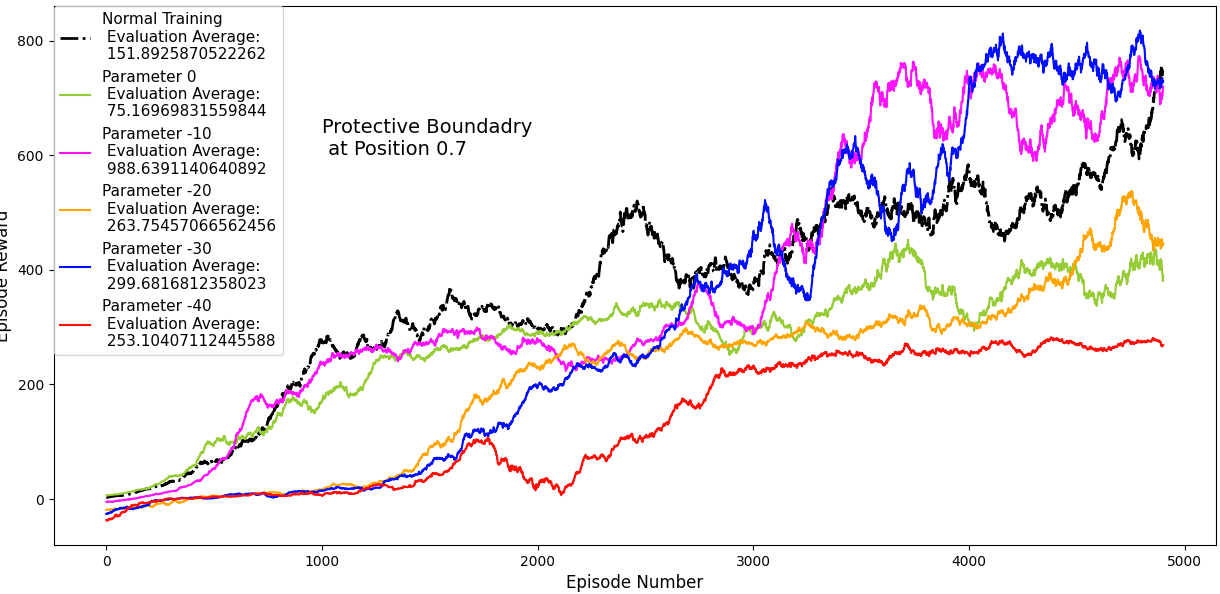
\includegraphics[width=\textwidth]{Walker_with_Boundary_at_0.7.png}
    \end{subfigure}
    \vspace*{0.0mm}
    \begin{subfigure}[b]{0.5\textwidth}
      \centering
      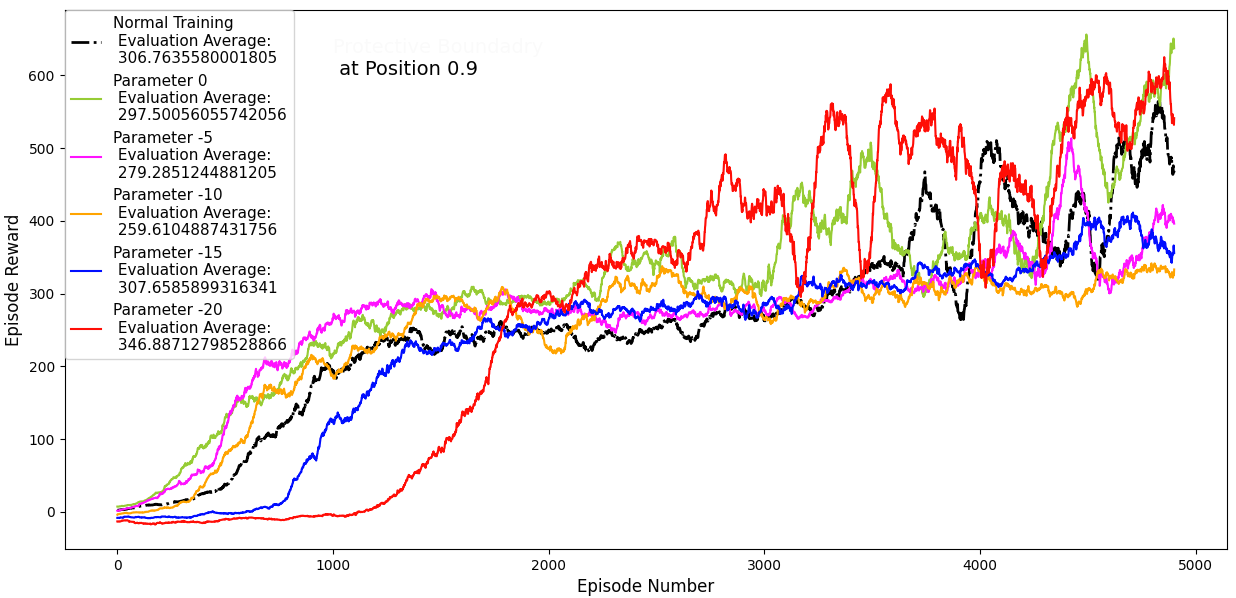
\includegraphics[width=\textwidth]{Walker_with_Boundary_at_0.9.png}
    \end{subfigure}
    \caption{Walker2D}
    \label{fig:Walker}
\end{figure}


\section{Conclution}

In this paper, we introduced the active boundary idea based on our observation of athletic training. Our proof of concept data suggests when the position and penalty associated with active boundary are set appropriately, accelerated learning can be achieved. Future research should focus on devising analytical tools that can systematically derive the best position and penalty for an active boundary.

Next step, we plan on extending the active boundary idea to the deep drone acrobat project \cite{Kaufmann2020DeepDA}. The training of drone acrobat is done in simulation and then transferred to a real-world drone controller. We think our active boundary method can greatly accelerate the training of drone acrobats. 

We believe our research opens door to a rich reservoir of potential researches along the direction of adapting proven human training techniques to RL environments. Human achieves superhuman feats not because of talent, but because of the meticulously engineered coaching tactics. Current researches in RL focus solely on the "athlete" side of the equation, i.e. how to build an efficient RL agent. But we feel "coach" is as important, if not more so.  For instance, the endgames training strategy was deployed to educate chess players. During the training phase, the agent should start the game middle way to amass experience with critical states, instead of wasting time on steps leading up to the critical position. Coaches also challenge athletes, pushing them to experience difficult situations. "Coach" could even be implemented by independent neural networks, in addition to the agent, and trained to "teach" better. All these should be investigated by future researches. 

\bibliographystyle{IEEEtran}
\bibliography{Bibliography}
%\printbibliography



\end{document}
